\noindent Unauthorized acts involving the use of radiological material, particularly in urban environments, is of national concern. The effects of a dirty bomb or radiological dispersal device being detonated in a densely-populated area would be catastrophic from a health, financial, and psychological standpoint. The ability of radiological search and recovery personnel to quickly to detect, localize and recover radioactive sources is critical for reducing this threat.
\\\\
The military normally breaks search and recovery down in to four operational areas:
\begin{itemize}
  \item Beyond Line of Sight (BLOS) - satellite and high altitude reconnaissance systems
  \item Far Area - fast moving airborne systems
  \item Near Area - ground vehicle, helicopter, and Unmanned Aerial Systems (UAS)
  \item Objective Area - Unmanned Ground Systems (UGS) and dismounted personnel
\end{itemize}
BLOS and Far Area operations are normally conducted by the Air Force while Near and Objective Area operations are conducted by Army and Marine Corps Technical forces or Special Operations Forces, depending on the threat, location, and operational availability of forces. Advances in UAS mounted detection has allowed for the collection of information in the Near Area that once could only be collected in the Objective Area. These advances and additional ones in UGS will minimize personnel exposure in the Objective Area. The goal of this work is to simulate a search and recovery scenario to explore the potential benefits of surface flux quantification. Specifically, to develop a quick and accurate localization method to minimize the exposure time of search and recovery personnel.

\subsection{Motivation}
\noindent In the early spring of 2018 the Defense Threat Reduction Agency (DTRA) invited numerous Universities, National Labs, and Commercial companies to partake in an Unmanned Search Technology Demonstration at Camp Roberts, CA. DTRA personnel placed an unknown source, of unknown activity, in a small village and participants were to detect and localize the source. Lawrence Berkeley National Laboratory (LBNL) demonstrated its Localization and Mapping Platform (LAMP).

\begin{figure}[!htb]
  \centering
  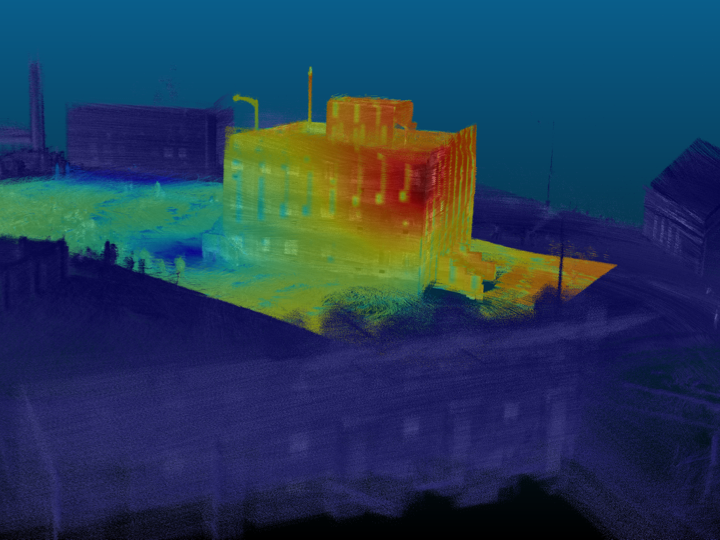
\includegraphics[width=\columnwidth]{images/Heatmap}
  \caption{Gamma "Heatmap" produced by LAMP at DTRA Unmanned Search Technology Demonstration}
  \label{fig:Heatmap}
\end{figure}

Fig. \ref{fig:Heatmap} displays the "Heatmap" produced by LAMP. While it is clear that the source is located near the corner of the building, which floor it is on is unclear. Furthermore, the source and its activity are still unknown. That information could drastically alter the methods used by recovery personnel. Quantification would allow for source identification by energy, activity calculation by flux, and precise localization filtering scattered gammas (filter by peak energy).
\\\\
The remainder of the paper describes methods for achieving this objective. Section \ref{sec:Model} details the development of the model and the tools used to conduct the simulations.  Section \ref{sec:Methodology} discusses how quantification and localization are simulated. Section \ref{sec:results} describes the results of the quantification and localization simulations. Finally, Section \ref{sec:conclusion} describes the limitations of this study and provides recommendations for future work.
